\documentclass[journal,12pt,twocolumn]{IEEEtran}
%
\usepackage{setspace}
\usepackage{gensymb}
\usepackage{xcolor}
\usepackage{caption}
\singlespacing

\usepackage[cmex10]{amsmath}
\usepackage{mathtools}
\usepackage{hyperref}
\usepackage{amsthm}
\usepackage{mathrsfs}
\usepackage{txfonts}
\usepackage{stfloats}
\usepackage{cite}
\usepackage{cases}
\usepackage{subfig}
\usepackage{longtable}
\usepackage{multirow}
\usepackage{enumitem}
\usepackage{mathtools}
\usepackage{listings}
\let\vec\mathbf

\DeclareMathOperator*{\Res}{Res}
\renewcommand\thesection{\arabic{section}}
\renewcommand\thesubsection{\thesection.\arabic{subsection}}
\renewcommand\thesubsubsection{\thesubsection.\arabic{subsubsection}}

\renewcommand\thesectiondis{\arabic{section}}
\renewcommand\thesubsectiondis{\thesectiondis.\arabic{subsection}}
\renewcommand\thesubsubsectiondis{\thesubsectiondis.\arabic{subsubsection}}

\hyphenation{op-tical net-works semi-conduc-tor}

\lstset{
language=Python,
frame=single, 
breaklines=true,
columns=fullflexible
}


\begin{document}
%

\theoremstyle{definition}
\newtheorem{theorem}{Theorem}[section]
\newtheorem{problem}{Problem}
\newtheorem{proposition}{Proposition}[section]
\newtheorem{lemma}{Lemma}[section]
\newtheorem{corollary}[theorem]{Corollary}
\newtheorem{example}{Example}[section]
\newtheorem{definition}{Definition}[section]
\newcommand{\BEQA}{\begin{eqnarray}}
\newcommand{\EEQA}{\end{eqnarray}}
\newcommand{\define}{\stackrel{\triangle}{=}}
\newcommand{\myvec}[1]{\ensuremath{\begin{pmatrix}#1\end{pmatrix}}}
\newcommand{\mydet}[1]{\ensuremath{\begin{vmatrix}#1\end{vmatrix}}}

\bibliographystyle{IEEEtran}

\providecommand{\nCr}[2]{\,^{#1}C_{#2}} % nCr
\providecommand{\nPr}[2]{\,^{#1}P_{#2}} % nPr
\providecommand{\pr}[1]{\ensuremath{\Pr\left(#1\right)}}
\providecommand{\qfunc}[1]{\ensuremath{Q\left(#1\right)}}
\providecommand{\sbrak}[1]{\ensuremath{{}\left[#1\right]}}
\providecommand{\lsbrak}[1]{\ensuremath{{}\left[#1\right.}}
\providecommand{\rsbrak}[1]{\ensuremath{{}\left.#1\right]}}
\providecommand{\brak}[1]{\ensuremath{\left(#1\right)}}
\providecommand{\lbrak}[1]{\ensuremath{\left(#1\right.}}
\providecommand{\rbrak}[1]{\ensuremath{\left.#1\right)}}
\providecommand{\cbrak}[1]{\ensuremath{\left\{#1\right\}}}
\providecommand{\lcbrak}[1]{\ensuremath{\left\{#1\right.}}
\providecommand{\rcbrak}[1]{\ensuremath{\left.#1\right\}}}

\theoremstyle{remark}
\newtheorem{rem}{Remark}
\newcommand{\sgn}{\mathop{\mathrm{sgn}}}

\providecommand{\abs}[1]{\ensuremath{\left\vert#1\right\vert}}
\providecommand{\res}[1]{\Res\displaylimits_{#1}}
\providecommand{\norm}[1]{\lVert#1\rVert}
\providecommand{\mtx}[1]{\mathbf{#1}}
\providecommand{\mean}[1]{\ensuremath{E\left[ #1 \right]}}
\providecommand{\fourier}{\overset{\mathcal{F}}{ \rightleftharpoons}}
\providecommand{\ztrans}{\overset{\mathcal{Z}}{ \rightleftharpoons}}

\providecommand{\system}{\overset{\mathcal{H}}{ \longleftrightarrow}}
\newcommand{\solution}{\noindent \textbf{Solution: }}
\providecommand{\dec}[2]{\ensuremath{\overset{#1}{\underset{#2}{\gtrless}}}}
\numberwithin{equation}{section}
\makeatletter
\@addtoreset{figure}{problem}
\makeatother

\let\StandardTheFigure\thefigure
\renewcommand{\thefigure}{\theproblem}

\def\putbox#1#2#3{\makebox[0in][l]{\makebox[#1][l]{}\raisebox{\baselineskip}[0in][0in]{\raisebox{#2}[0in][0in]{#3}}}}
\def\rightbox#1{\makebox[0in][r]{#1}}
\def\centbox#1{\makebox[0in]{#1}}
\def\topbox#1{\raisebox{-\baselineskip}[0in][0in]{#1}}
\def\midbox#1{\raisebox{-0.5\baselineskip}[0in][0in]{#1}}

\vspace{3cm}

\title{ Pingala Series }
\author{ Sumanth N R }
\maketitle

\tableofcontents

\renewcommand{\thefigure}{\theenumi}
\renewcommand{\thetable}{\theenumi}

\bigskip

\begin{abstract}
This manual provides a simple introduction to Transforms
\end{abstract}



\section{JEE 2019}
Let 
\begin{align}
	a_n &= \frac{\alpha^{n}-\beta^{n}}{\alpha - \beta}, \quad n \ge 1 \\
	b_n &= a_{n-1} + a_{n+1}, \quad n \ge 2, \quad b_1 =1
	\label{eq:10-orig-diff}
\end{align}

Verify the following using a python code.

\begin{enumerate}[label=\thesection.\arabic*,ref=\thesection.\theenumi]
\item \begin{align}
	\sum_{k=1}^{n}a_k = a_{n+2}-1, \quad n \ge 1
\end{align}
\item \begin{align}
	\sum_{k=1}^{\infty}\frac{a_k}{10^k} =\frac{10}{89}
\end{align}
\item \begin{align}
	b_n =\alpha^n + \beta^n, \quad n \ge 1
\end{align}
\item \begin{align}
	\sum_{k=1}^{\infty}\frac{b_k}{10^k} =\frac{8}{89}
\end{align}
\end{enumerate}

\solution
	The following code verifies all the equations
	\begin{lstlisting}
wget https://raw.githubusercontent.com/Sigma1084/EE3900/master/pingala/code/Ex1_verify.py
	\end{lstlisting}



\section{Pingala Series}

\begin{enumerate}[label=\thesection.\arabic*,ref=\thesection.\theenumi]

\item The {\em one sided} $Z$-transform of $x(n)$ is defined as 
	\begin{align}
		X^{+}(z) = \sum_{n = 0}^{\infty}x(n)z^{-n}, \quad z \in \mathbb{C}
		\label{eq:one-Z}
	\end{align}

\item The {\em Pingala} series is generated using the difference equation 
	\begin{align}
		\begin{split} \label{eq:10-pingala}
			x(n+2) = x\brak{n+1} +& x\brak{n} \\
			x(0) = x(1) =& 1, n \ge 0
		\end{split}
	\end{align}
	Generate a stem plot for $x(n)$. \\
	\solution The following code generates the plot
	\begin{lstlisting}
wget https://raw.githubusercontent.com/Sigma1084/EE3900/master/pingala/code/Ex2_pingala.py
	\end{lstlisting}
	\begin{figure}[!htp]
		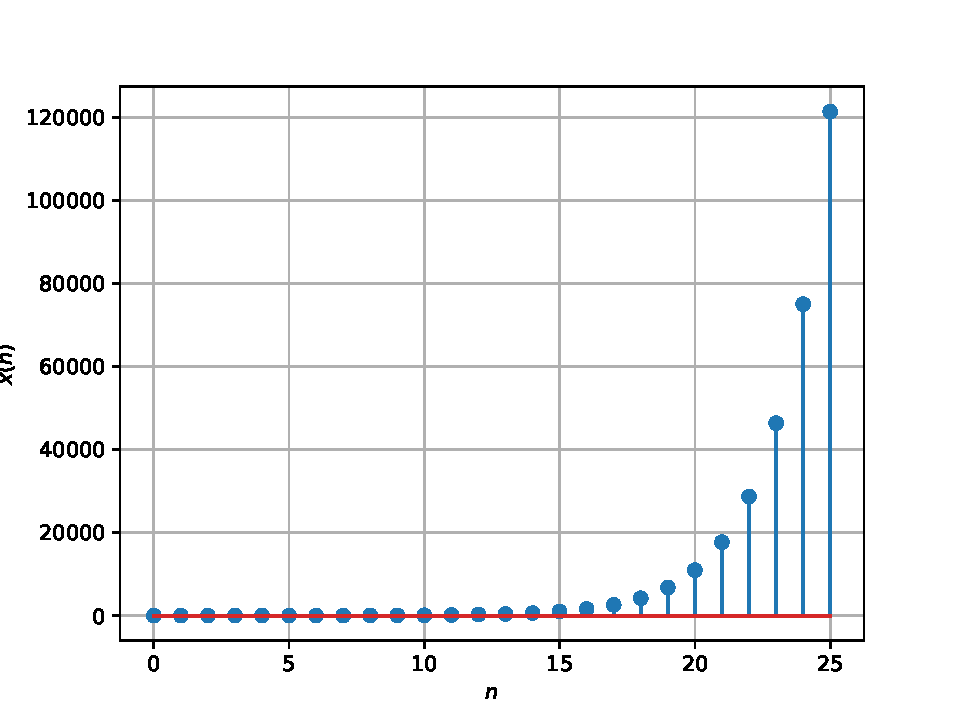
\includegraphics[width=\columnwidth]{../figs/x_n.pdf}
		\caption{Plot of $x(n)$}
		\label{fig:x-n}
	\end{figure}


\newpage


\item Find $X^{+}(z)$. \\
	\solution Taking the {\em one-sided} $Z$-transform on both sides of \eqref{eq:10-pingala}
	\[
		\mathcal{Z}^+\sbrak{x(n + 2)} = \mathcal{Z}^+\sbrak{x(n + 1)} + \mathcal{Z}^+\sbrak{x(n)}
	\]
	\begin{align*}
		\implies &z^2X^+(z) - z^2 - z = \ zX^+(z) - z + X^+(z) \\
		\implies &\brak{z^2 - z - 1} X^+(z) = \ z^2 \\
		\implies &X^+(z) = \frac{1}{1 - z^{-1} - z^{-2}}
	\end{align*}
	\begin{align}
		X^+(z) = \frac{1}{\brak{1 - \alpha z^{-1}}\brak{1 - \beta z^{-1}}}, \quad |z| > |\alpha|
		\label{eq:X-z}
	\end{align}
	Here $\alpha$ and $\beta$ are the roots of the characteristic equation of \eqref{eq:10-pingala} and $|z| > |\alpha|$ is the region of convergence of $X^+(z)$. \\
	(w.l.o.g, $|\alpha| > |\beta|$ is assumed)


\item Find $x(n)$. \\
	\solution Expanding $X^+(z)$ in \eqref{eq:X-z} using partial fractions, we get
	\begin{align*}
		X^+(z) &= \frac{1}{\brak{\alpha - \beta}z^{-1}}\sbrak{\frac{1}{1 - \alpha z^{-1}} - \frac{1}{1 - \beta z^{-1}}} \\
			&= \frac{1}{\brak{\alpha - \beta}}\sum_{n = 0}^{\infty}\brak{\alpha^n - \beta^n}z^{-n} \\
			&= \sum_{n = 1}^\infty \frac{\alpha^{n} - \beta^{n}}{\alpha - \beta}z^{-n + 1} \\
			&= \sum_{n = 0}^\infty \frac{\alpha^{n + 1} - \beta^{n + 1}}{\alpha - \beta}z^{-n}
	\end{align*}
	\begin{align}
		x(n) = \frac{\alpha^{n + 1} - \beta^{n + 1}}{\alpha - \beta}u(n) = a_{n + 1}u(n)
		\label{eq:x-n}
	\end{align}


\item Sketch
	\begin{align}
		y(n) = x\brak{n-1} + x\brak{n+1}, \quad n \ge 0
		\label{eq:10-orig-diff-rev}
 	\end{align}
	 \solution The following code generates the plot
	 \begin{lstlisting}
 wget https://raw.githubusercontent.com/Sigma1084/EE3900/master/pingala/code/Ex2_pingala.py
	 \end{lstlisting}
	 \begin{figure}[!htp]
		 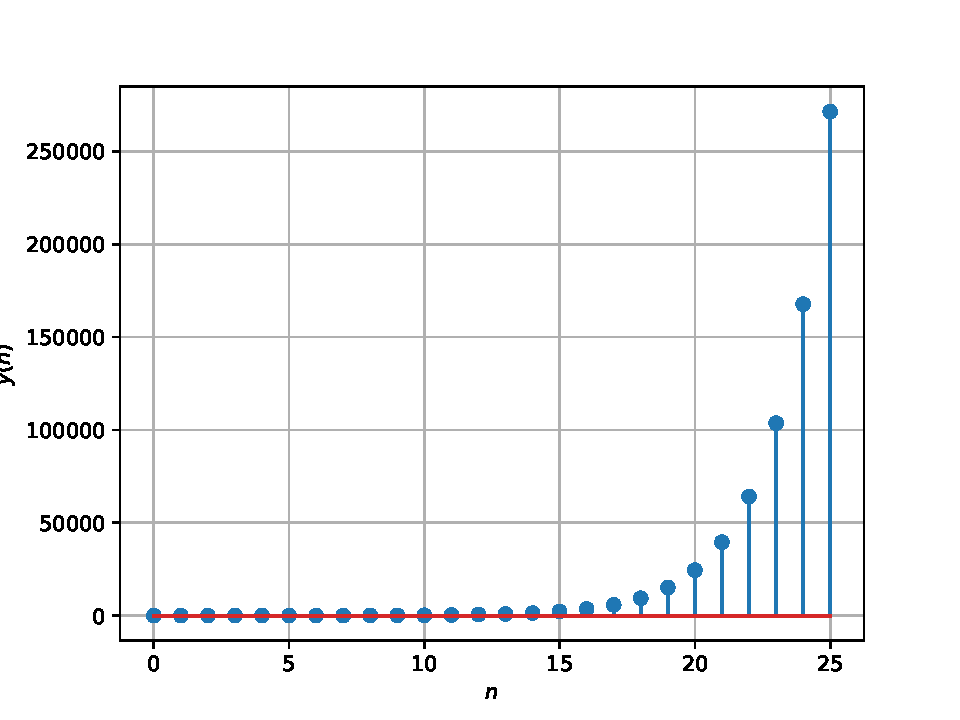
\includegraphics[width=\columnwidth]{../figs/y_n.pdf}
		 \caption{Plot of $y(n)$}
		 \label{fig:y-n}
	 \end{figure}


\item Find $Y^{+}(z)$. \\
	\solution
	Taking the one-sided $Z$-transform on both sides of \eqref{eq:10-orig-diff-rev},
	\[
		\mathcal{Z}^+\sbrak{y(n)} = \mathcal{Z}^+\sbrak{x(n + 1)} + \mathcal{Z}^+\sbrak{x(n - 1)}
	\]
	\begin{align}
		Y^+(z) =& \ zX^+(z) - zx(0) + z^{-1}X^+(z) + zx(-1) \nonumber \\
		=& \ \frac{z + z^{-1}}{1 - z^{-1} - z^{-2}} - z \nonumber \\
		Y^+(z) =& \ \frac{1 + 2z^{-1}}{1 - z^{-1} - z^{-2}}, \quad |z| > |\alpha| \label{eq:Y-z}
	\end{align}
	\ensuremath{\big( x(-1) = 0 \text{ since } x(n) = 0 \ \forall\ n < 0 \big)}

\item Find $y(n)$. \\
	\solution Using \eqref{eq:Y-z},
	\begin{align*}
		Y^+(z) &= (1 + 2z^{-1}) \ X^+(z) \\
			&= (1 + 2z^{-1})\sum_{n = 0}^{\infty}x(n)z^{-n} \\
			&= \sum_{n = 0}^{\infty}x(n)z^{-n} + \sum_{n = 1}^{\infty}2x(n - 1)z^{-n} \\
			&= x(0) + \sum_{n = 1}^{\infty}\brak{x(n) + 2x(n - 1)}z^{-n} \\
			&= x(0) + \sum_{n = 1}^{\infty}\brak{x(n + 1) + x(n - 1)}z^{-n}
	\end{align*}

	\begin{align*}
		\implies \quad & y(0) = x(0) = 1 \\
			& \forall n > 0 \quad y(n) = x(n+1) + x(n-1) \\
			& \quad \quad \quad \quad \quad \quad = a_{n+2} + a_n = b_{n+1}
	\end{align*}

	$\alpha$ and $\beta$ are the roots of the characteristic equation of \eqref{eq:10-pingala}, $z^2 - z - 1 = 0$ \\
	(w.l.o.g, $|\alpha| > |\beta|$ is assumed) \\
	$\implies \alpha\beta = -1 \quad \text{and} \quad \alpha + \beta = 1$

	\begin{align}
		y(n) &= \frac{\brak{\alpha^{n + 2} - \beta^{n + 2}} + \brak{\alpha^{n} + \beta^{n}}}{\alpha - \beta} \nonumber \\
			&= \frac{\brak{\alpha^{n + 2} - \beta^{n + 2}} - \alpha\beta\brak{\alpha^{n} + \beta^{n}}}{\alpha - \beta} \nonumber \\
			&= \frac{\brak{\alpha - \beta}\brak{\alpha^{n + 1} + \beta^{n + 1}}}{\alpha - \beta} \nonumber \\
		y(n) &= \alpha^{n + 1} + \beta^{n + 1} \label{eq:y-n}
	\end{align}

	Thus, $y(n) = \alpha^{n + 1} + \beta^{n + 1}$ for $n \geq 0$ as $\alpha + \beta = 1$. \\
	Comparing \eqref{eq:y-n} with the definition of $b_n$, we see that $y(n) = b_{n + 1}$.
	\begin{align}
		\implies b_{n+1} = y(n) = \alpha^{n + 1} + \beta^{n + 1} \quad \forall n > 0 \label{op:3}
	\end{align}

\end{enumerate}



\section{Power of the Z transform}

\begin{enumerate}[label=\thesection.\arabic*,ref=\thesection.\theenumi]


\item Show that
	\begin{align}
		\sum_{k=1}^{n}a_k = 
		\sum_{k=0}^{n-1}x(n) = x(n)*u(n-1)
	\end{align}
	\solution
	Using \eqref{eq:x-n}, and the definition of convolution,
	\begin{align*}
		\sum_{k=1}^{n}a_k &= \sum_{k=0}^{n-1}a_{k+1} = \sum_{k=-\infty}^{n-1}a_{k+1} \ u(k)\\
		&= \sum_{k=-\infty}^{n-1}x(k) \\ 
		&= \sum_{k=-\infty}^{\infty}x(k) \ u(n-1-k)\\
		&= u(n-1) * x(n) \\
		\implies \sum_{k=1}^{n}a_k &= x(n) * u(n-1)
	\end{align*}


\item Show that
	\begin{align}
		a_{n+2}-1, \quad n \ge 1
	\end{align}
	can be expressed as 
	\begin{align}
		\sbrak{x\brak{n+1}-1}u\brak{n}
	\end{align}
	\solution
	Using \eqref{eq:x-n}, and the definition of $u(n)$
	\begin{align*}
		& \ a_{n+2} - 1 & n \ge 1 \\
		=& \ \sbrak{x\brak{n+1}-1} & n \ge 0 \\
		=& \ \sbrak{x\brak{n+1}-1}u\brak{n}
	\end{align*}


\item Show that
	\begin{align}
		\sum_{k=1}^{\infty}\frac{a_k}{10^k}= 
		\frac{1}{10}\sum_{k=0}^{\infty}\frac{x\brak{k}}{10^k} =\frac{1}{10}X^{+}\brak{{10}}
	\end{align}
	\solution Using the definitions of  $x(n)$ \eqref{eq:x-n} and $X^+(z)$ \eqref{eq:X-z},
	\begin{align}
		\sum_{k=1}^{\infty}\frac{a_k}{10^k} &= \frac{1}{10}\sum_{k = 0}^{\infty}\frac{a_{k+1}}{10^k} \nonumber \\
		&= \frac{1}{10}\sum_{k = 0}^{\infty}\frac{x(k)}{10^k} \nonumber \\
		&= \frac{1}{10}X^+(10) \nonumber \\
		&= \frac{1}{10}\times\frac{1}{1 - \frac{1}{10} - \frac{1}{100}} \nonumber \\
		\implies \sum_{k=1}^{\infty}\frac{a_k}{10^k} &= \frac{10}{89} \label{op:2}
	\end{align}


\item Show that
	\begin{align}
		\alpha^n + \beta^n, \quad n \ge 1
		\label{eq:b-n-q}
	\end{align}
	can be expressed as 
	\begin{align}
		w(n) =\brak{\alpha^{n+1} + \beta^{n+1}}u(n)
	\end{align}
	and find $W(z)$. \\
	\solution Putting $n = n+1$ in \eqref{eq:b-n-q}, we get
	\begin{align*}
		& \alpha^{n} + \beta^{n} & n \ge 1\\
		=& \ \alpha^{n+1} + \beta^{n+1} & n \ge 0 \\
		w(n) :=& \ \brak{\alpha^{n+1} + \beta^{n+1}} u(n) = y(n)
	\end{align*}
	Since we know $w(n) = y(n)$, we can use \eqref{eq:Y-z} to find $W(z)$
	\begin{align*}
		W(z) =& \sum_{n=-\infty}^\infty w(n) = \sum_{n=0}^\infty y(n)\\
		=& \ Y^+(z) = \frac{1 + 2z^{-1}}{1 - z^{-1} - z^{-2}}, \quad |z| > |\alpha| \\
	\end{align*}


\item Show that
	\begin{align}
		\sum_{k=1}^{\infty}\frac{b_k}{10^k} =
		\frac{1}{10}\sum_{k=0}^{\infty}\frac{y\brak{k}}{10^k} =\frac{1}{10}Y^{+}\brak{{10}}
	\end{align}
	\solution Using the definitions of  $y(n)$ \eqref{eq:y-n} and $Y^+(z)$ \eqref{eq:Y-z},
	\begin{align}
		\sum_{k=1}^{\infty}\frac{b_k}{10^k}
		&= \frac{1}{10}\sum_{k = 0}^{\infty}\frac{b_{k+1}}{10^k} \nonumber \\
		&= \frac{1}{10}\sum_{k = 0}^{\infty}\frac{y(k)}{10^k} \nonumber \\
		&= \frac{1}{10}Y^+(10) \nonumber \\
		&= \frac{1}{10} \times \frac{1 + 2\frac{1}{10}}{1 - \frac{1}{10} - \frac{1}{100}} \nonumber \\
		\implies \sum_{k=1}^{\infty}\frac{a_k}{10^k} &= \frac{12}{89} \label{op:4} \\ \nonumber
	\end{align}


\item Solve the JEE 2019 problem. \\
	\solution We know that
	\begin{align}
		\sum_{k = 1}^{n}a_k = x(n)*u(n - 1)
	\end{align}
	But
	\begin{align*}
		&x(n)*u(n - 1) \ztrans X(z)z^{-1}U(z) \\
		&= \frac{z^{-1}}{\brak{1 - z^{-1} - z^{-2}}\brak{1 - z^{-1}}} \\
		&= z\sbrak{\frac{1}{1 - z^{-1} - z^{-2}} - \frac{1}{1 - z^{-1}}} \\
		&\ztrans z\sum_{n = 0}^{\infty}\brak{x(n) - 1}z^{-n} \\
		&= \sum_{n = 0}^{\infty}\brak{x(n) - 1}z^{-n + 1} \\
		&= \sum_{n = 0}^{\infty}\brak{x(n + 1) - 1}z^{-n} \\
	\end{align*}
	From \eqref{eq:x-n}, we get
	\begin{align}
		\sum_{k = 1}^{n}a_k = a_{n+2} - 1 \label{op:1}
	\end{align}
	Using \eqref{op:1}, \eqref{op:2}, \eqref{op:3} and \eqref{op:4}, we can conclude that Options 1, 2, 3 are right and Option 4 is wrong.

\end{enumerate}


\end{document}